\documentclass[11pt,twoside,onecolumn,a4paper]{article}
%% put "oui" in the following line to see labels and other debugging text
\newcommand{\imprimeTexteSecret}{non}
%% put "oui" in the following line to see solutions
\newcommand{\imprimeTexteCache}{non}
\usepackage{lebArticle,ulem,cancel}
%
\newcommand{\cor}[2]{\cancel{#1} {\red #2}}
%

\input{lebstuff}
\begin{document}
\title{
\begin{minipage}[c]{10cm}Errata
\\
Performance Evaluation of Computer and Communication Systems\\
\vspace{2cm}
%
\end{minipage}
%
%
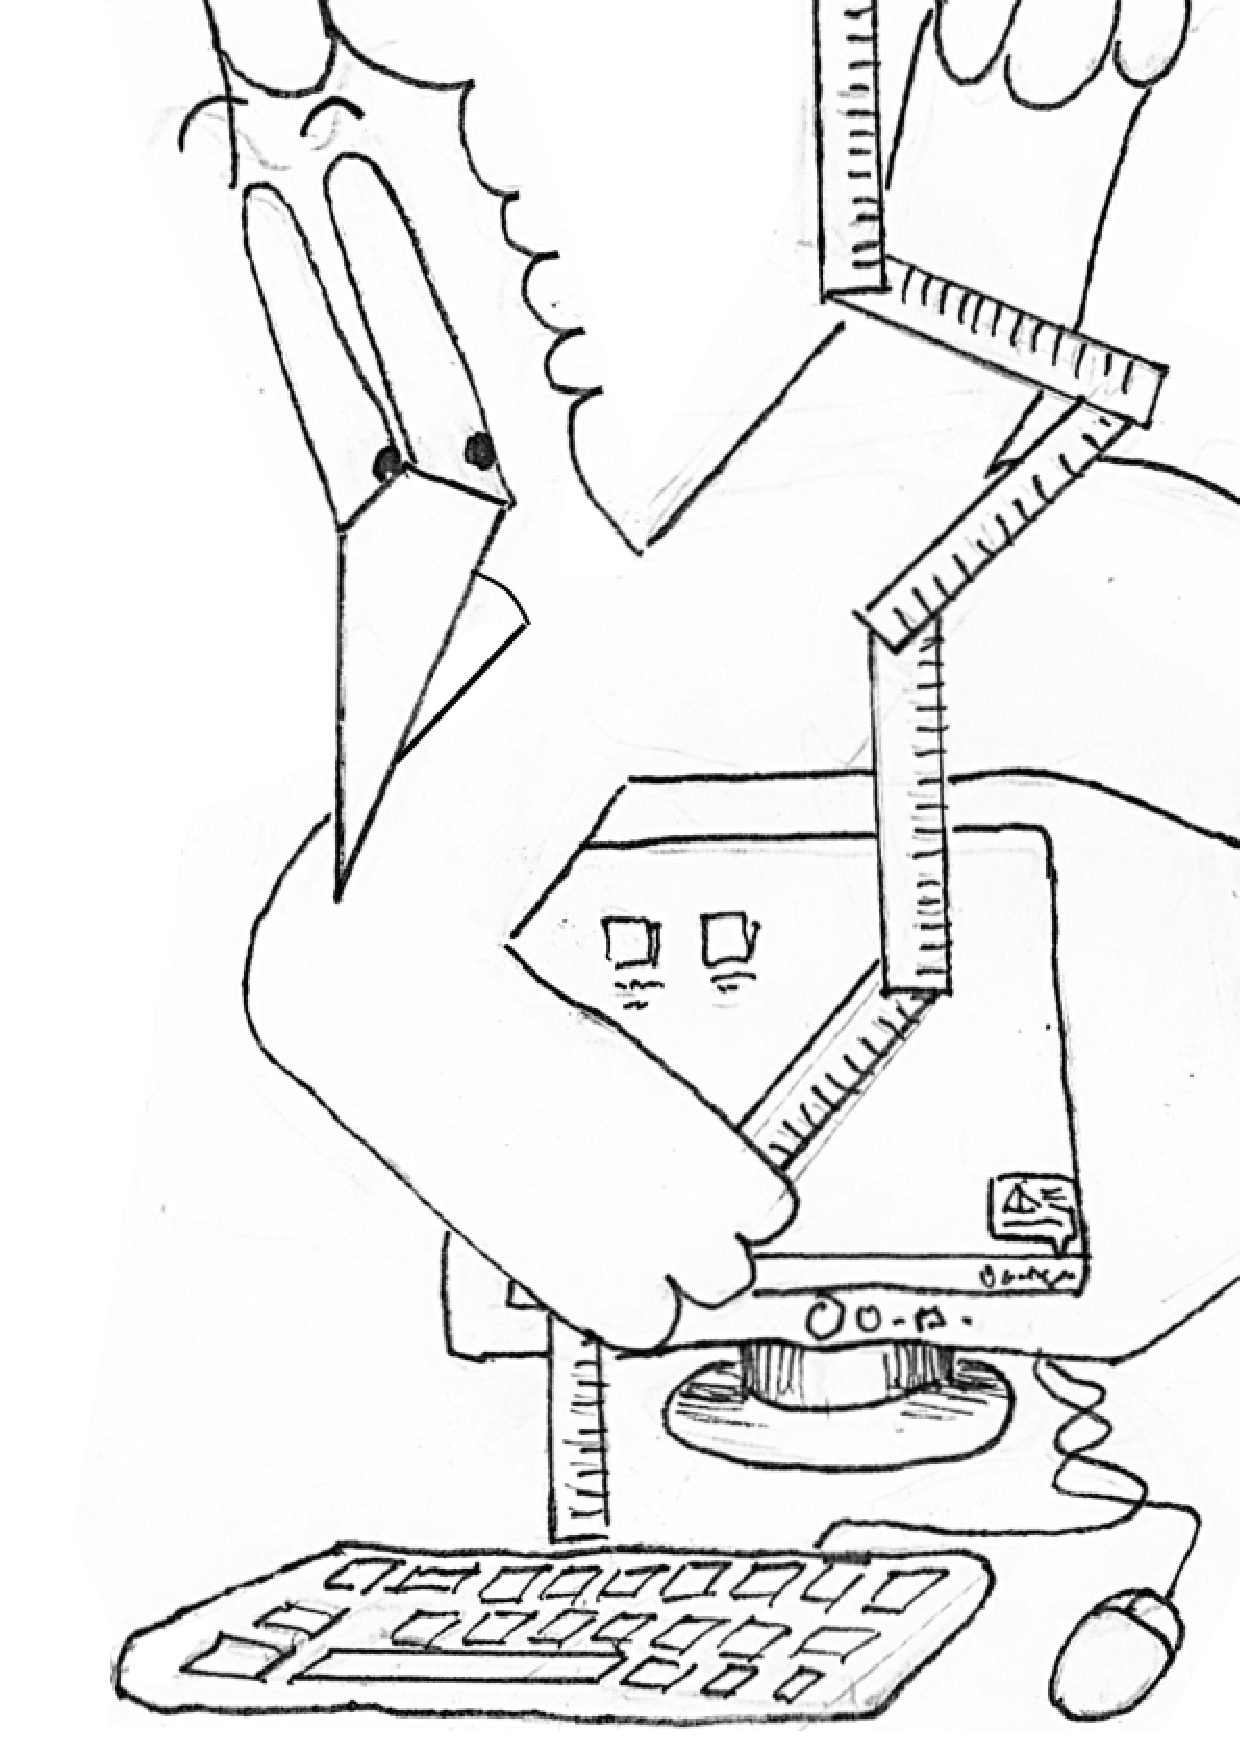
\includegraphics[scale=0.1]{scouacMesureOrdi.pdf}}
\author{Jean-Yves Le Boudec}
\date{\today\\Available at \pro{https://leboudec.github.io/perfeval/}}
\maketitle
This is the list of known bugs, with credits, in the publisher's version (ISBN: 978-2-940222-40-7
2010). These bugs are fixed in the online version. Page references are for the publisher's version. A number of bug fixes were done in earlier stages by Irina Baltcheva,
 Manuel Flury,
 Olivier Gallay,
 Assane Gueye,
 Paul Hurley,
 Ruben Merz,
 Bo\v{z}idar Radunovi\'{c},
 Gianluca Rizzo,
 Slavi\v{s}a Sarafijanovi\'{c},
 Milan Vojnovi\'{c},
 Utkarsh Upadhyay
 and
 Jonas Wagner who are here gratefully acknowledged.

If you see residual bugs in the online
version please send me a mail !


 \subsection*{Chapter 1}
 \begin{itemize}
 \item Page 5, Example 1.5 $\lceil x \rceil$ is the \cor{floor}{ceiling} of $x$ [Roger Vion].
 \end{itemize}

 \subsection*{Chapter 2}
 \begin{itemize}
\item Eq. 2.25 p. 39: $[\hat{\sigma}_n\sqrt{\cor{\frac{\zeta}{n-1}}{\frac{n-1}{\xi}}},\hat{\sigma}_n \sqrt{\cor{\frac{\xi}{n-1}}{\frac{n-1}{\zeta}}}]$ [Patrick Loiseau].

\item Page 27, after Eq (2.7):
from an exponential distribution, gap $\approx$\cancel{ $0.74$}{ \red${0.37}$} [Jeong-woo Cho].

$\mbox{ gap}_{\mbox{th}}=\sqrt{\cor{2 \over \pi}{1 \over 2\pi}}\frac{\sigma}{\mu}$

\item Page 30, caption of Figure 2.5:
The maximum distance (plain line) is equal to \cancel{$\sqrt{2}$} {\red$1\over \sqrt{2}$} times
  the maximum vertical deviation (dashed line) [Jeong-woo Cho].

\item Page 31 ``A measure of fairness is the largest euclidian
distance (the gap) from the Lorenz curve to the
diagonal, rescaled by its maximum value
\cancel{$(\sqrt{2}$)}
{\red $\left(1\over \sqrt{2}\right)$}
\item Page 32, last comment
$\mbox{Gini}_{\mbox{th}} = 2\int_0^{\cor{\infty}{1}} \lp q - L(q)\rp dq
 =1- 2\int_0^{\cor{\infty}{1}} L(q) dq$ [Jeong-woo Cho].
 \item  Page 37: Note that, for small values of $n$, no confidence
interval is possible at the levels $\cor{0.95\%}{0.95}$ or $\cor{0.99\%}{0.99}$ [Jeong-woo Cho].
 \end{itemize}

 \subsection*{Chapter 3}
 \begin{itemize}
 \item Page 74, Example 3.5 $f'(\mu) = i - (I-i)= 2{\red i}-I$ [Roger Vion].
 \item Page 77, Theorem 3.3. (4): and $g=\sum_{j,k}u_jG_{j,k}\cor{u_k^2}{u_k}=\sum_k\lp\sum_j u_j K_{j,k}\rp^2$
 \item Page 74: If $I$ is odd, $f$
decreases on $(-\infty, y_{(\cor{2I}{I}+1)/2}]$ and increases on
$[y_{(\cor{2I}{I}+1)/2}, +\infty)$, thus is minimum for $\mu=
y_{(\cor{2I}{I}+1)/2}$, which is the sample median.  [Jeong-woo Cho].
\item Page 85 Caption of Table 3.2 $\Gamma()$ is
the gamma function, defined as $\Gamma(x)=\int_0^{\infty}{\red e^{-t} }
t^{x-1} dt$ [Roger Vion]
\item Page 91 The standard Weibull distribution with exponent $c$
has support on $[0,\infty ) $ and is defined by its CDF equal
to $1-\cor{e^{\lp  x ^c \rp}}{e^{-\lp  x ^c \rp}}$ [Jlien Harbulot].
\item Page 94, changed the identifier of the mixture probability $p$ to $q$ in order to avoid confusion with the Pareto index $p$ in the following example.
\item Page 97: Indeed, if $X_i$ are \cor{idd}{iid} with finite variance [Roger Vion].
 \item Pages 99-100 A mobile moves in some area
from one point to the next \sout{from one point to the next} [Roger Vion].
\end{itemize}


  \subsection*{Chapter 4}
 \begin{itemize}

 \item Page 116, before equation (4.3):

 The likelihood
ratio test has a rejection region of the form
$l_{\vx}(H_1)-l_{\vx}(H_0)> \cor{k}{K}$ for some constant \cor{$k$}{$K$}.

After eq (4.3), add:
for some other constant $k$.

 \item Page 117, $(X_k, Y_k)$ is
independent of $(X_{\cor{k}{k'}}, Y_{k'})$ [Jeong-woo Cho]

\item Page 117, Eq. (4.7)
 replace $\bmat{c}n!\\n_1!...n_k!\emat$ by $\frac{n!}{n_1!...n_k!}$

\item Pages 117 \cor{$N_i$}{$\vec{N}$} comes from ... (2 times)

     \item Page 119: \cor{The pivot is}{A pivot is a function of the data whose probability distribution under $H_0$ is the same for all $\theta \in\Theta_0$. For this test the pivot is} [Jeong-woo Cho]
         \item Page 116
         \bearn
\hat{\sigma}_1^{2}&=&\frac{1}{n}\sum_i (x_i^{\cor{2}{}}-\hat{\mu}_n^+)^2
 \eearn
 \item Page 126, Example 4.13
   \begin{quote}
   \texttt{Parameter Set 1 pchi2 = 0.0002854}\\
   \texttt{Parameter Set \cor{1}{2} pchi2 = 0.02731}\\
   \texttt{Parameter Set \cor{1}{3} pchi2 = 0.6669}
   \end{quote}
  \end{itemize}

 \subsection*{Chapter 5}
 \begin{itemize}
 \item Page 154, Example 5.5 we only need to \cor{fil}{fit} one parameter (namely $\sigma$) [Roger Vion].
 \item Page 155, Equation (5.20)
  \ben
 \hat{\gamma}_t = \frac{1}{n} \sum_{s=1}^{n-t}(X_{\cor{n}{s}+t}-\bar{X})(X_{\cor{n}{s}}-\bar{X})
\een

\item Page 168,
The idea is to keep a running estimate \cor{estimate}{} $\hat{m}_t$... [Roman Rudnik].

  \end{itemize}


  \subsection*{Chapter 6}
 \begin{itemize}
 \item Page 178, Figure 6.1, Panel (a) text on top: $\mu_F=\cor{ 0.096 }{ 0.0096 }$.
 \item Page 196, Corollary 6.1 to the unique index {\red $n\geq 0$} such that.
 \item Page 190, footnote \cor{ 0.95 }{ 0.05 } [Jeong-woo Cho].
 \item Page 192, first line: The period of a random number generator should be much \cor{ smaller }{ larger } [Jeong-woo Cho].
 \item Page 194, just before Example 6.11: $x\in\cor{\;\I}{\;I}$ [Jeong-woo Cho].
 \end{itemize}

  \subsection*{Chapter 7}
 \begin{itemize}
 \item Page 217, We break the integral in Eq.(7.2) into pieces
    corresponding to the intervals \cor{$[T_{n}, T_{n+1} )$}{$[T_{n-1}, T_{n})$}.
 \item Page 226, eqs (7.21) and (7.22), opening parentheses are missing after the $\E$ signs.
 \item Page 231, Example 7.8: $f^0_T(\cor{t}{s})=\lambda e^{-\lambda s}$
 \item Page 234, \cor{$\Delta X_t $}{ $\Delta_t$ } [Jeong-woo Cho].
 \item Page 234, eq. (7.34) \cor{$\ind{t \leq T_n} $}{ $\ind{t \geq T_n}$ } [Jeong-woo Cho].
 \item Page 234, eq. (7.35) \cor{$\ind{\ind{t \leq T_n^j}} $}{ $\ind{\ind{t \geq T_n^j}}$ } [Jeong-woo Cho].
 \item Page 235, \cor{$\Delta X $}{ $\Delta_t$ } [Jeong-woo Cho].
 \item Page 241, It is often
presented in the context of renewal processes {\red(where interarrival times are i.i.d.)}[Jeong-woo Cho].
\item page 242, footnote, is independent of \cor{$m$}{$n$} [Jeong-woo Cho].
 \end{itemize}

 \subsection*{Chapter 8}
 \begin{itemize}
 \item Page 265, Example 8.1 $D(t)=r{\red(}  t -d(0){\red)} - \Delta$ [Roger Vion].
 \item Page 266, footnote \cor{between $A(t)$ and $A'(t)$}{between $(D1)$ and $(D2)$}[Jeong-woo Cho].
\item Page 269, Theorem 8.3 \cor{a $B$}{an $s$}-server queue [Jeong-woo Cho].
\item Page 271, Figure 8.5: a loopback arrow is missing from CPU to CPU.
\item Page 271, Legend of Figure 8.5, delete ``$n$ attendants serve customers."
\item Page 272, Eq. (8.2) \cor{$Z$}{$\bar{Z}$}[Jeong-woo Cho].
\item Page 275, Eq. (8.5) $\calL_W(s) = \frac{s(1-\rho)}{s -\la +{\red\la} \calL_S(s)}$ [Jeong-woo Cho].
\item Page 275, Eq. (8.7) $\kappa= \frac{1}{2}\left(1+\frac{\sigma^2_S}{\bar{S}^2}\right) =
 \frac{1}{2}\left(1+\mbox{CoV}_S\cor{}{^2}\right)$
\item Page 276 One approach is based on \cor{a}{} the following [Jeong-woo Cho].
\item Page 291, Example 8.6 Classes 1, 2 or 3
represent \cor{internal}{external} jobs and class 4 internal
jobs. [Jeong-woo Cho].
\item Page 292, Example 8.6 Jobs of classes 1, 2 or 3 are \cor{internal}{external}
    jobs. [Jeong-woo Cho].
\item Page 303, Theorem 8.11 $\cor{\vK}{K}_{\calC}$ is
the number of customers of chain $\calC$
\item Page 315 $\frac{1}{\tilde{\theta}_{\calC}}
      \sum_{s \in \calS, c \in \calC} \theta^s_c q^{s,s'}_{c,c'}
   \mif \cor{c}{c'} \in \calC$  [Jeong-woo Cho].
\item Page 336 The mean value analysis equations are
(Section 8.6.\cor{5}{7}) [Jeong-woo Cho].





 \end{itemize}

\subsection*{Annex C}
 \begin{itemize}
   \item Page 369, Example C.3: as seen in Example \cor{C.12}{C.1}.

 \end{itemize}

\end{document}
